% kdtree.tex
% revised 10/12/2009
% $Header: acmtr.tex,v 1.5 2/14/96 11:07:57 boyland Exp $

\documentclass[acmjacm]{acmtrans2m}

\let\mycounter\setcounter

%&t&{\tt #}&
%&v&\verb|#|&

\acmVolume{2}
\acmNumber{3}
\acmYear{09}
\acmMonth{12}

\usepackage[utf8]{inputenc}
\usepackage{graphicx}
\usepackage{amsmath}
\usepackage{algorithmic}
\usepackage{algorithm}
\usepackage{url}


\newcommand{\BibTeX}{{\rm B\kern-.05em{\sc i\kern-.025em b}\kern-.08em
    T\kern-.1667em\lower.7ex\hbox{E}\kern-.125emX}}
\newcommand{\titulo}{Adaptive Load Balancing for MMOG servers using kd-trees}
\newcommand{\autores}{Carlos Eduardo B. Bezerra, João L. D. Comba and Cláudio F. R. Geyer}
%\markboth{Leslie Lamport et al.}{Preparing Articles for the ACM 
\markboth{Carlos Eduardo Benevides Bezerra et al.}{\titulo}

\title{\titulo}
\author{CARLOS EDUARDO B. BEZERRA, JOÃO L. D. COMBA and CLÁUDIO F. R. GEYER\\Universidade Federal do Rio Grande do Sul}


\begin{abstract}
In Massively Multiplayer Online Games (MMOGs) there is a great demand for high bandwidth connections with irregular access patterns.
Such irregular demand is due to the fact that participants in these games, which can vary from few hundreds to several tens of thousands, 
often occupy the virtual environment of the game in many different ways with varying densities. Therefore, there is
a great need for decentralized architectures with multiple servers that employ load balancing algorithms to manage regions of the virtual environment. In such systems, each player only connects to the server that manages the region where the player is located, whereas each  server is responsible for mediating the interaction between all pairs of players connected to it. Devising the proper
load balancing algorithm to take into account spatial and variable occupation is a challenging problem, which
requires adaptive (and possibly dynamic) partitioning of the virtual environment. 
%Some work has already been made in this direction, but with a geometric algorithm, more appropriate than those found in the literature, it should be possible to reduce the distribution granularity without compromising the rebalancing time, or even reducing it. 
In this work, we propose the use of a kd-tree for partitioning the game environment into regions, and
dynamically adjust the resulting subdivision based on the distribution of avatars in the virtual environment. We compared our algorithm to competing approaches found in the literature and show that our algorithm performed better in most aspects we analyzed.


%MMOGs (massively multiplayer online games) are applications that require high bandwidth connections to work properly. This demand for bandwidth is specially critical on the servers that host the game. This happens because the typical number of simultaneous participants in this kind of game varies from a few hundreds to several tens of thousands, and the server is the one responsible for mediating the interaction between every pair of players connected to it. To deal with this problem, decentralized architectures with multiple servers have been proposed, where each server manages a region of the virtual environment of the game. Each player, then, connects only to the server that manages the region where he is playing. However, to distribute the load among the servers, it is necessary to devise an algorithm for partitioning the virtual environment. In order to readjust the load distribution during the game, this algorithm must be dynamic. Some work has already been made in this direction, but with a geometric algorithm, more appropriate than those found in the literature, it should be possible to reduce the distribution granularity without compromising the rebalancing time, or even reducing it. In this work, we propose the use of a kd-tree for dividing the virtual environment of the game into regions, each of which being designated to one of the servers. The split coordinates of the regions are adjusted dynamically according to the distribution of avatars in the virtual environment. We compared our algorithm to some approaches found in the literature and the simulation results show that our algorithm performed better in most aspects we analyzed.

\end{abstract}

\category{C.2.4}{Computers Systems Organizations}{Computer-Communication Networks}%
[Distributed Systems]

\category{I.3.5}{Computing Methodologies}{Computer Graphics}[Computational Geometry and Object Modeling]

\terms{Algorithms, Management, Performance}

\keywords{distributed server, kd-trees, load balancing, MMOGs}


\newcommand{\misccite}[2]{#1. Available at: \textless#2\textgreater. Last time accessed: 24 jul. 2009}
\newcommand{\gamecite}[2]{\misccite{#1}{#2}}

\begin{document}


\setcounter{page}{1}



{\let\setcounter\mycounter
    \begin{bottomstuff}
    	Author's address: Carlos Eduardo B. Bezerra, Programa de Pós-Graduação em Computação,
		Instituto de Informática, Universidade Federal do Rio Grande do Sul,
		Caixa Postal 15064, 91501-970, Porto Alegre - RS - Brasil.
%		\newline
%		Start of a second footnote ...
    \end{bottomstuff}
}

\maketitle


\section{Introduction}

The main characteristic of Massively Multiplayer Online Games (MMOGs) is the large number of players interacting simultaneously, which currently can reach up to tens of thousands \cite{schiele2007rpp}. Client-server architectures are often configured to allow communication among players, with the server intermediating the communication between each pair of players. To allow player interaction, each player sends commands to the server, which calculates the new game state and propagates back to all players impacted by the state change. This mechanism can lead to many state update messages sent by the server, which may be quadratic on the number of players when all players interact among themselves. Therefore, the cost of maintaining a centralized infrastructure like this is high when many players are used, thus restricting the MMOG market to large companies with enough resources to pay the upkeep of the server.

In order to reduce this cost, several decentralized solutions have been proposed. Possible solutions include peer-to-peer networks \cite{schiele2007rpp,rieche2007ppb,hampel2006ppa,elrhalibi2005abm,iimura2004zfg,knutsson2004pps} or distributed servers
\cite{ng2002msa,chertov:olb,lee2003sdl,assiotis2006dam},
which are composed of low-cost nodes connected through the Internet. Common to both approaches is the fact that the ``world'', or virtual environment of the game is divided into regions which are managed by a server (or a group of peers). Each of these regions must not violate its capacity, and thus must not have more content than the load imposed on the corresponding server.

Players are assigned to servers based on their location. When an \emph{avatar} (representation of the player in the virtual environment) is located in a region, the player controlling that avatar connects to the server associated to that region. This server becomes responsible for processing the input from that player and for sending update messages in response. If a server becomes overloaded due to an excessive number of avatars in its region, a new partitioning of the virtual environment must be calculated to alleviate the overloaded server.

Usually, the virtual environment is divided into relatively smaller cells, which are grouped into regions and distributed among the servers. However, this approach has a severe limitation in its granularity, since the cells have fixed size and position. Using more elaborate partitioning algorithms allows better player distribution among different servers, which rely on traditional data structures generally used in geometric algorithms \cite{samet2005}. In this work, we use a kd-tree to dynamically perform the spatial partitioning of the virtual environment. When a server is overloaded, it triggers the load balancing algorithm, which changes the limits of each region by changing the split coordinates stored in the kd-tree. We validate our proposal with several simulations and compare the results to previous work that uses the cell division technique.

The text is organized as follows: in section \ref{context}, some related works are described; in section \ref{sec:proposal}, the algorithm proposed here is presented in detail; in the sections \ref{sec:simul} and \ref{sec:result}, we present, respectively, the simulation details and its results and, in section \ref{sec:conc}, the conclusions of this work are presented.


\section{Related Work}
\label{context}

Different authors have tried to address the problem of spatial partitioning the virtual environment in MMOGs for better distribution among multiple servers \cite{ahmed2008mol,bezerra2009lbs}. The simplest solution is to use a static division into cells of fixed size and position, with cells grouped into regions, and each region delegated to one of the servers (Figure \ref{fig:cells}). When one server becomes overloaded, it looks for another server to absorb one or more cells of its cells.

\begin{figure}[!t]
	\centering
	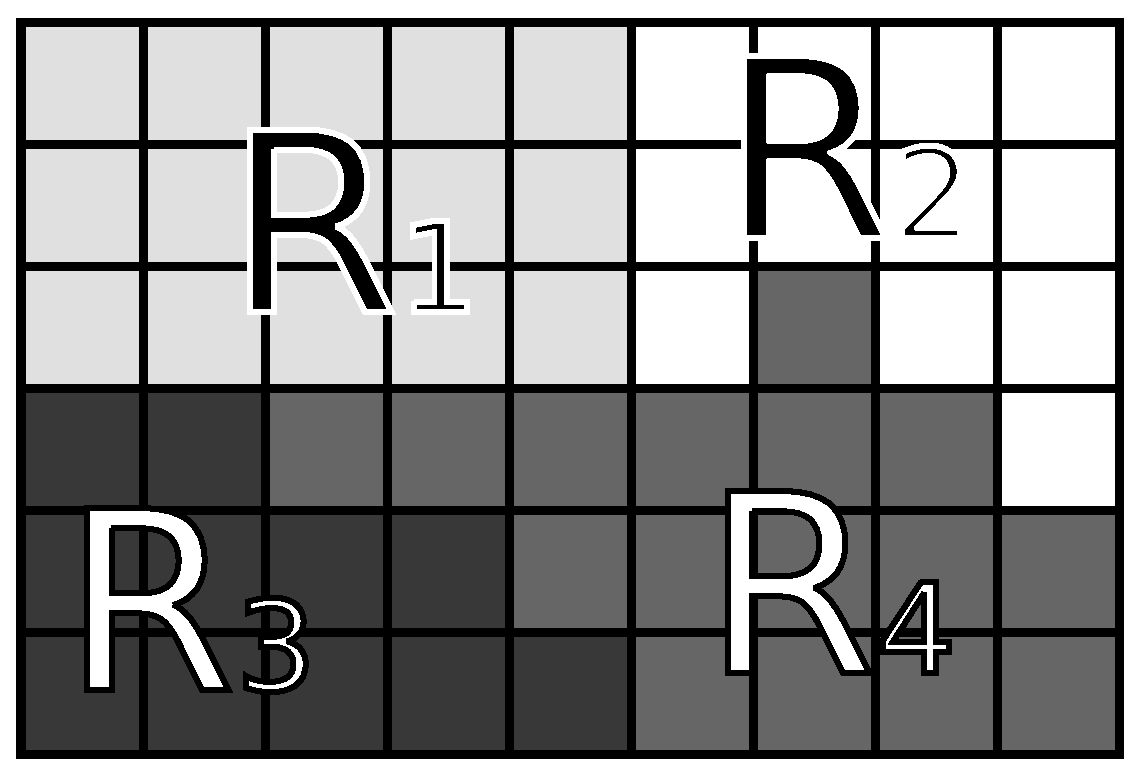
\includegraphics[width=0.4\linewidth]{images/macromicro}
	\caption{Division into cells and grouping into regions}
	\label{fig:cells}
\end{figure}

In the work of \cite{ahmed2008mol} a cell-oriented load balancing model is proposed. Their algorithm first enumerate all clusters of cells that are managed by the overloaded server. The smallest cluster is found, and selected the cell from this cluster that has the least interaction with other cells on the same server -- the interaction between two cells A and B is defined by the authors as the number of pairs of avatars interacting with each other, one from A and the other from B. The selected cell is transferred to the least loaded server, considering ``load'' as the bandwidth used to send state updates to the players whose avatars are positioned in the cells managed by that server. This process is repeated until the server is no longer overloaded or there is no more servers capable of absorbing more load -- in this case, one option could be to reduce the frequency at which state update messages are sent to the players, as suggested by \cite{bezerra2008a3}.

\begin{figure}[!t]
	\centering
	\includegraphics[width=0.7\linewidth]{images/grafo}
	\caption{Graph representation of the virtual environment}
	\label{fig:graph}
\end{figure}

In \cite{bezerra2009lbs}, it is also proposed the division into cells. To perform the division, the environment is represented by a graph, where each vertex represents a cell (Figure \ref{fig:graph}). Every edge in the graph connects two vertices representing neighboring cells. The weight of a vertex is the server's bandwidth occupied to send state updates to the players whose avatars are in the cell represented by that vertex. The interaction between any two cells define the weight of the edge connecting the corresponding vertices. To form the regions, the graph is partitioned using a greedy algorithm: starting from the heaviest vertex, at each step it is added the vertex connected by the heaviest edge to any of the vertices already selected, until the total weight of the partition of the graph -- defined as the sum of the vertices' weights -- reaches a certain threshold related to the total capacity of the server that will receive the region represented by that partition of the graph.

Although this approach works, there is a serious limitation on the distribution granularity it can achieve. If a finer granularity is desired, it is necessary to use very small cells, increasing the number of vertices in the graph that represents the virtual environment and, consequently, the time required to perform the balancing. Besides, the control message containing the list of cells designated to each server also becomes longer. Thus, it may be better to use another approach to perform the partitioning of the virtual environment, possibly using a more suitable data structure, such as the kd-tree \cite{bentley1975mbs}.

This kind of data structure is generally used in computer graphics. However, as in MMOGs there is geometric information -- such as the position of the avatars in the environment --, space partitioning trees can be used. Moreover, we cand find in the literature techniques for keeping the partitions defined by the tree with a similar ``load''. In \cite{luque2005bpc}, for example, it is sought to reduce the time needed to calculate the collisions between pairs of objects moving through space. The authors propose the use of a BSP (binary space partitioning) tree to distribute the objects in the scene (Figure \ref{fig:bsp}). Obviously, if each object of a pair is completely inserted in a different partition, they do not collide and there is no need to perform a more complex test for this pair. Assuming an initial division, it is proposed by the authors a dynamic readjustment of the tree as objects move, balancing their distribution on the leaf-nodes of the tree and, therefore, minimizing the time required to perform the collision detection. Some of the ideas proposed by the authors may be used in the context of load balancing between servers in MMOGs.

\begin{figure}[!t]
	\centering
	\includegraphics[width=0.3\linewidth]{images/bsp}
	\caption{Space partitioning using a BSP tree}
	\label{fig:bsp}
\end{figure}

\section{Proposed approach}
\label{sec:proposal}

The load balancing approach proposed here is based on two criteria: first, the system should be considered heterogeneous (i.e. every server may have a different amount of resources) and, second, the load on each server is \emph{not} proportional to the number of players connected to it, but to the amount of bandwidth required to send state update messages to them.

This choice is due to the fact that every player sends commands to the server at a constant rate, so the number of messages received by the server per unit time grows linearly with the number of players, whereas the number of state update messages sent by the server may be quadratic, in the worst case.

As mentioned in the introduction, to divide the environment of the game into regions, we propose the utilization of a data structure known as kd-tree. The vast majority of MMOGs, such as World of Warcraft \cite{worldofwarcraft}, Ragnarok \cite{ragnarok} and \mbox{Lineage II} \cite{lineage2}, despite having three-dimensional graphics, the simulated world -- cities, forests, swamps and points of interest in general -- in these games is mapped in two dimensions. Therefore, we propose to use a kd-tree with \mbox{k = 2}.

Each node of the tree represents a region of the space and, moreover, in this node it is stored a split coordinate. Each one of the two children of that node represents a subdivision of the region represented by the parent node, and one of them represents the sub-region before the split coordinate and the other one, the sub-region containing points whose coordinates are greater than or equal to the split coordinate. The split axis (in the case of two dimensions, the axes $x$ and $y$) of the coordinate stored alternates for every level of the tree -- if the first level nodes store x-coordinates, the second level nodes store y-coordinates and so on. Every leaf node also represents a region of the space, but it does not store any split coordinate. Instead, it stores a list of the avatars present in that region. Finally, each leaf node is associated to a server of the game. When a server is overloaded, it triggers the load balancing, which uses the kd-tree to readjust the split coordinates that define its region, reducing the amount of content managed by it.

Every node of the tree also stores two other values: capacity and load of the subtree. The load of a non-leaf node is equal to the sum of the load of its children. Similarly, the capacity of a non-leaf node is equal to the sum of the capacity of its children nodes. For the leaf nodes, these values are the same of the server associated to each one of them. The tree root stores, therefore, the total weight of the game and the total capacity of the server system.

In the following sections, it will be described the construction of the tree, the calculation of the load associated with each server and the proposed balancing algorithm.

\subsection{Building the kd-tree}

To make an initial space division, it is constructed a balanced kd-tree. For this, we use the recursive function shown in Algorithm \ref{alg:buildtree} to create the tree.

\begin{algorithm}
\caption{node::build\_tree(id, level, num\_servers)}
\label{alg:buildtree}
\begin{algorithmic}
	\IF{id + $2^{level} \ge num\_servers$ }
		\STATE $left\_child \leftarrow right\_child \leftarrow NIL$;
		\STATE return;
	\ELSE
		\STATE $left\_child \leftarrow$ new\_node();
		\STATE $left\_child.parent \leftarrow$ \textbf{this};
		\STATE $right\_child \leftarrow$ new\_node();
		\STATE $right\_child.parent \leftarrow$ \textbf{this};
		\STATE $left\_child$.build\_tree$(id, level + 1, num\_servers)$;
		\STATE $right\_child$.build\_tree$(id + 2^{level}, level + 1, num\_servers)$;
	\ENDIF
\end{algorithmic}
\end{algorithm}

\begin{figure}[!t]
	\centering
	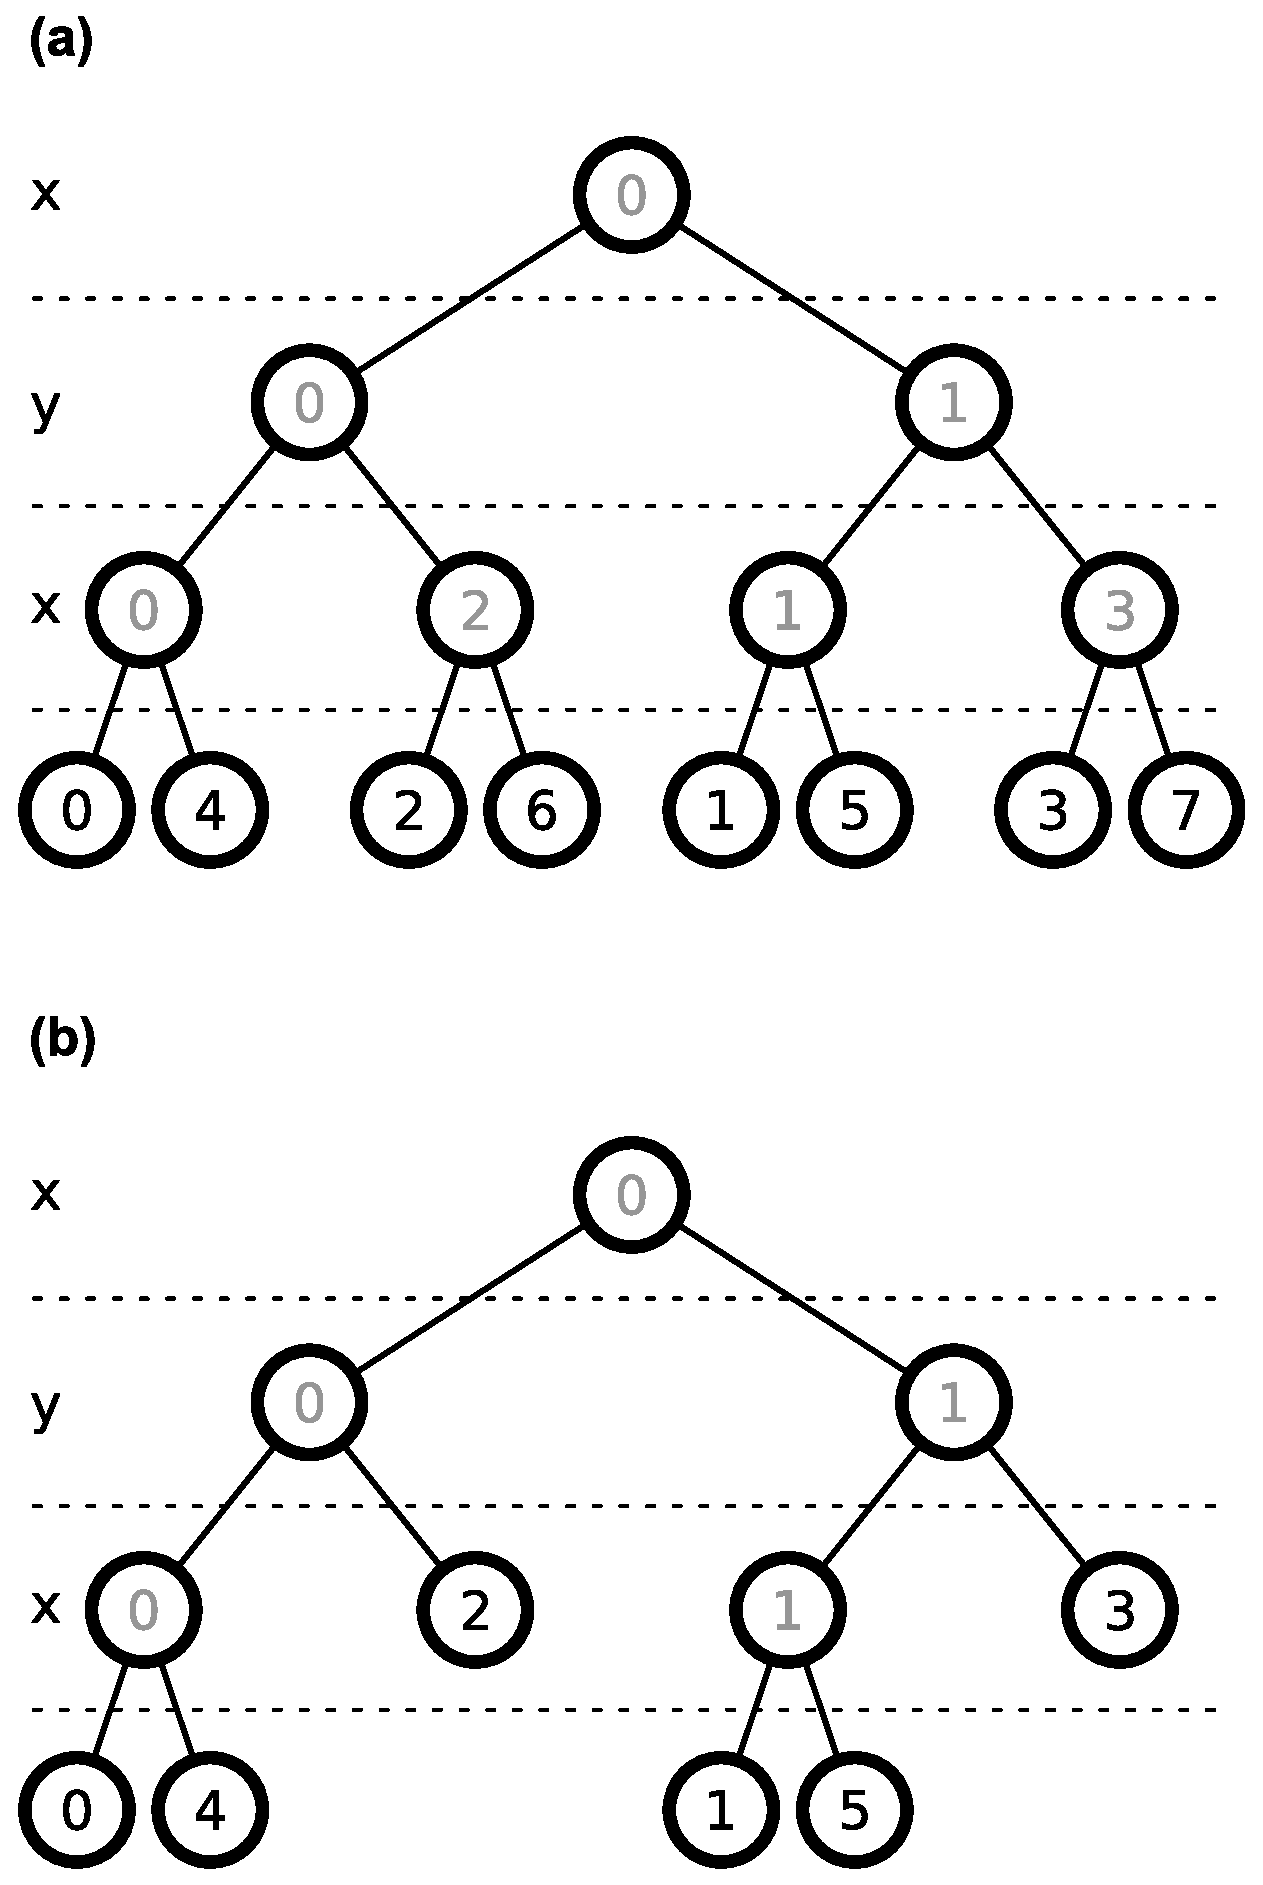
\includegraphics[width=\linewidth]{images/kdtree}
	\caption{Balanced kd-trees built with the described algorithm}
	\label{fig:kdtree}
\end{figure}

In Algorithm \ref{alg:buildtree}, the $id$ value is used to calculate whether each node has children or not and, in the leaf nodes, it determines the server associated to the region represented by each leaf of the tree. The purpose of this is to create a balanced tree, where the number of leaf nodes on each of the two sub-trees of any node differs, in the maximum, by one. In Figure \ref{fig:kdtree} (a), we have a full kd-tree formed with this simple algorithm and, in Figure \ref{fig:kdtree} (b), an incomplete kd-tree with six-leaf nodes. As we can see, every node of the tree in (b) has two sub-trees whose number of leaf nodes differs by one in the worst case.

\subsection{Calculating the load of avatars and tree nodes}

The definition of the split coordinate for every non-leaf node of the tree depends on how the avatars will be distributed among the regions. An initial idea might be to distribute the players among servers, so that the number of players on each server is proportional to the bandwidth of that server. To calculate the split coordinate, it would be enough to simply sort the avatars in an array along the axis used ($x$ or $y$) by the tree node to split the space and, then, calculate the index in the vector, such that the number of elements before this index is proportional to the capacity of the left child and the number of elements from that index to the end of the array is proportional to the capacity of the right child (Figure \ref{fig:vector}). The complexity of this operation is $O(nlogn)$, due to the sorting of avatars.

\begin{figure}
  \centering
  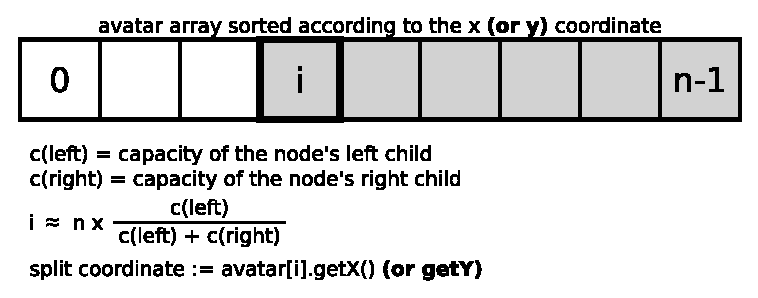
\includegraphics[width=0.8\linewidth]{images/vector}
  \caption{A load splitting considering only the number os avatars}
  \label{fig:vector}
\end{figure}

However, this distribution is not optimal, for the load imposed by the players depends on how they are interacting with one another. For example, if the avatars of two players are distant from each other, there will be probably no interaction between them and, therefore, the server will need only to update every one of them about the outcome of his own actions -- for these, the growth in the number of messages is linear with the number of players. On the other hand, if the avatars are close to each other, each player should be updated not only about the outcome of his own actions but also about the actions of every other player -- in this case, the number of messages may grow quadratically with the number of players \mbox{(Figure \ref{fig:load})}. For this reason, it is not sufficient only to consider the number of players to divide them among the servers.

\begin{figure}
  \centering
  
\includegraphics[width=0.8\linewidth]{images/carga}
  \caption{Relation between avatars and load}
  \label{fig:load}
\end{figure}

A more appropriate way to divide the avatars is by considering the load imposed by each one of them on the server. A brute-force method for calculating the loads would be to get the distance separating each pair of avatars and, based on their interaction, calculate the number of messages that each player should receive by unit of time. This approach has complexity $O(n^2)$. However, if the avatars are sorted according to their coordinates on the axis used to divide the space in the kd-tree, this calculation may be performed in less time.

For this, two nested loops are used to sweep the avatars array, where each of the avatars contains a $load$ variable initialized with zero. As the vector is sorted, the inner loop may start from an index before which it is known that no avatar $a_j$ has relevance to that being referenced in the outer loop, $a_i$. It is used a variable $begin$, with initial value of zero: if the coordinate of $a_j$ is smaller than that of $a_i$, with a difference greater than the maximum view range of the avatars, the variable $begin$ is incremented. For every $a_j$ which is at a distance smaller than the maximum view range, the $load$ of $a_i$ is increased according to the relevance of $a_j$ to $a_i$. When the inner loop reaches an avatar $a_j$, such that its coordinate is greater than that of $a_i$, with a difference greater than the view range, the outer loop moves immediately to the next step, incrementing $a_i$ and setting the value of $a_j$ to that stored in $begin$ (Figure \ref{fig:sweep}).

Let $width$ be the length of the virtual environment along the axis used for the splitting; let also $radius$ be the maximum view range of the avatars, and $n$, the number of avatars. The number of relevance calculations, assuming that the avatars are uniformly distributed in the virtual environment is \mbox{$O(m \times n)$}, where $m$ is the number of avatars compared in the internal loop, i.e. \mbox{$m = \frac{2 \times radius \times n}{width}$}. The complexity of sorting the avatars along one of the axes is $O(nlogn)$. Although it is still quadratic, the execution time is reduced significantly, depending on the size of the virtual environment and on the view range of the avatars. The algorithm could go further and sort each set of avatars $a_j$ which are close (in one of the axes) to $a_i$ according to the other axis and, again, perform a sweep eliminating those which are too far away, in both dimensions. The number of relevance calculations would be \mbox{$O(p \times n)$}, where $p$ is the number of avatars close to $a_i$, considering the two axes of coordinates, i.e. \mbox{$p = \frac{(2 \times radius)^2 \times n}{width \times height}$}. In this case, $height$ is the extension of the environment in the second axis taken as reference. Although there is a considerable reduction of the number of relevance calculations, it does not pay the time spent in sorting the sub-array of the avatars selected for each $a_i$. Adding up all the time spent on sort operations, it would be obtained a complexity of: \mbox{$O(nlogn + n \times mlogm)$}.

\begin{figure}
  \centering
  \includegraphics[width=0.8\linewidth]{images/sweep}
  \caption{Sweep of the sorted array of avatars}
   \label{fig:sweep}
\end{figure}

After calculating the load generated by each avatar, this value is used to define the load on each leaf node and, recursively, on the other nodes of the kd-tree. To each leaf node a server and a region of the virtual environment are assigned. The load of the leaf node is equal to the server's bandwidth used to send state updates to the players controlling the avatars located in its associated region. This way, the load of each leaf node is equal to the sum of the weights of the avatars located in the region represented by it.

\subsection{Dynamic load balancing}

Once the tree is built, each server is associated to a leaf node -- which determines a region. All the state update messages to be sent to players whose avatars are located in a region must be sent by the corresponding server. When a server is overloaded, it may transfer part of the load assigned to it to some other server. To do this, the overloaded server collects some data from other servers and, using the kd-tree, it adjusts the split coordinates of the regions.

Every server maintains an array of the avatars located in the region managed by it, sorted according to the $x$ coordinate. Also, each element of the array stores a pointer to another element, forming a chained list that is ordered according to the $y$ coordinated of the avatars (Figure \ref{fig:vectorxlisty}). By maintaining a local sorted avatar list on each server, the time required for balancing the load is somewhat reduced, for there will be no need for the server performing the rebalance to sort again the avatar lists sent by other servers. It will need only to merge all the avatars lists received from the other servers in an unique list, used to define the limits of the regions, what is done by changing the split coordinates which define the space partitions.

\begin{figure}
  \centering
  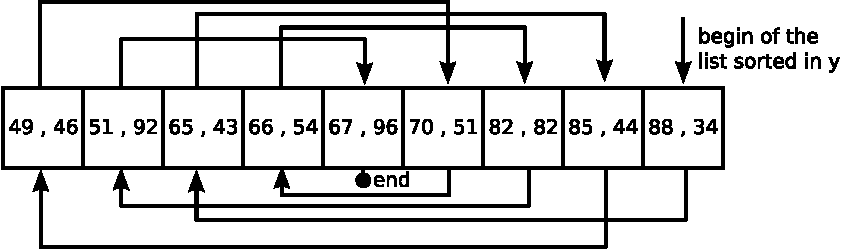
\includegraphics[width=0.9\linewidth]{images/vectorxlisty}
  \caption{Avatar array sorted by x, containing a list sort by y}
   \label{fig:vectorxlisty}
\end{figure}

When the overloaded server initiates the rebalance, it runs an algorithm that traverses the kd-tree, beginning from the leaf node that defines its region and going one level up at each step until it finds an ancestor node with a capacity greater then or equal to the load. While this node is not found, the algorithm continues recursively up the tree until it reaches the root. For each node visited, a request for the information about all the avatars and the values of load and capacity is sent to the servers represented by the leaf nodes of the sub-tree to the left of that node (Figure \ref{fig:ancestors}). With these data, and its own list of avatars and values of load and capacity, the overloaded server can calculate the load and capacity of its ancestral node visited in the kd-tree, which are not known beforehand -- these values are sent on-demand to save up some bandwidth of the servers and to keep the system scalable.

\begin{figure}
  \centering
  \includegraphics[width=0.8\linewidth]{images/ancestors}
  \caption{Search for an ancestor node with enough resources}
   \label{fig:ancestors}
\end{figure}

Reaching an ancestral node with capacity greater than or equal to the load -- or the root of the tree, if no such node is found -- the server that initiated the balance adjusts the split coordinates of the kd-tree nodes. For each node, it sets the split coordinate in a way such that the avatars are distributed according to the capacity of the node's children. For this, it is calculated the load fraction that should be assigned to each child node. The avatar list is then swept, stopping at the index $i$ such that the total load of the avatars before $i$ is approximately equal to the value defined as the load to be designated to the left child of the node whose split coordinate is being calculated (Figure \ref{fig:balancenode}). The children nodes have also, in turn, their split coordinates readjusted recursively, so that they are checked for validity -- the split coordinate stored in a node must belong to the region defined by its ancestors in the kd-tree -- and readjusted to follow the balance criteria defined.

\begin{figure}
  \centering
  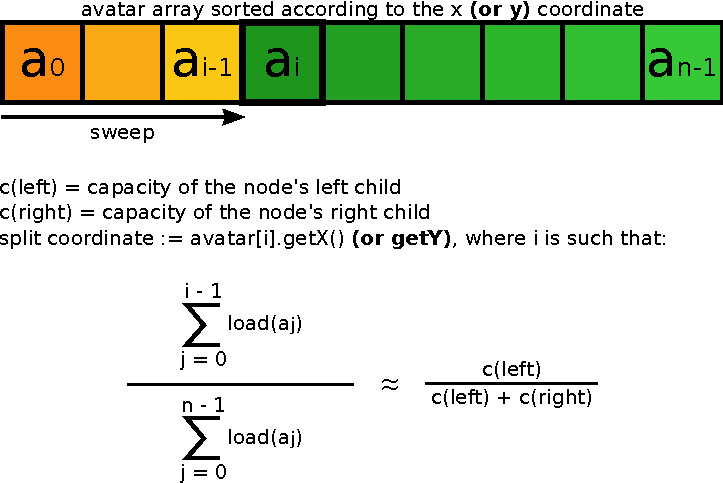
\includegraphics[width=0.8\linewidth]{images/balancenode}
  \caption{Division of an avatar list between two brother nodes}
   \label{fig:balancenode}
\end{figure}

As the avatar lists received from the other servers are already sorted along both axes, it is enough to merge these structures with the avatar list of the server which initiated the rebalance. Assuming that each server already calculated the weight of each avatar managed by it, the rebalance time is  $O(nlogS)$, where $n$ is the number of avatars in the game and $S$ is the number of servers. The communication cost is $O(n)$, caused by the sending of data related to te $n$ avatars. The merging of all avatar lists has $O(n)$ complexity, for the avatars were already sorted by the servers. At each level of the kd-tree, $O(n)$ avatars are swept in the worst case, in order to find the $i$ index whose avatar's coordinate will be used to split the regions defined by each node of the tree (Figure \ref{fig:balancenode}). As this is a balanced tree with $S$ leaf nodes, it has a height of $\lceil logS \rceil$.

\section{Simulations}
\label{sec:simul}

To evaluate the proposed dynamic load balancing algorithm, a virtual environment across which many avatars moved was simulated. Starting from a random point in the environment, each avatar moved according to the random waypoint model \cite{bettstetter2004spr}. To force a load imbalance and stress the algorithms tested, we defined some \emph{hotspots} -- points of interest to which the avatars moved with a higher probability than to other parts of the map. This way, a higher concentration of avatars was formed in some areas. Although the movement model used is not very realistic in terms of the way the players move their avatars in real games, it was only used to verify the load balance algorithms simulated. For each algorithm tested, we simulated two situations: one with the presence of hotspots and one without hotspots.

The proposed approach was compared to the ones presented in section \ref{context}, from other authors. However, it is important to observe that the model employed by \cite{ahmed2008mol} considers hexagonal cells, while in our simulations we used rectangular cells. Furthermore, the authors considered that there is a transmission rate threshold, which is the same for all servers in the system. As we assume a heterogenous system, their algorithm was simulated considering that each server has its own transmission rate threshold, depending on the upload bandwidth available in each one of them. However, we kept what we consider the core idea of the authors' approach, which is the selection of the smallest cell cluster managed by the overload server, then choosing that cell with the lowest interaction with other cells of the same server, and finally the transferring of this cell to the least loaded server. Besides Ahmed's algorithm, we also simulated some of the ones proposed in \cite{bezerra2009lbs} -- Progrega and BFBCT.

The simulated virtual environment consisted of a two-dimensional space, with 750 moving avatars, whose players were divided among eight servers ($S_1, S_2, ..., S_8$), each of which related to one of the regions determined by the balancing algorithm. For the cell-oriented approaches simulated, the space was divided into a \mbox{15 $\times$ 15} cell grid, or 225 cells. The capacity of each server $S_i$ was equal to $i \times 20000$, forming a heterogeneous system. This heterogeneity allowed us to evaluate the load balancing algorithms simulated according to the criterion of proportionality of the load distribution on the servers.

In addition to evaluate the algorithms according to the proportionality of the load distribution, it was also considered the number of player migrations between servers. Each migration involves a player connecting to the new server and disconnecting from the old one. This kind of situation may occur in two cases: the avatar moved, changing the region in which it is located and, consequently, changing the server to which its player is connected; or the avatar was not moving and still its player had to migrate to a new server. In the latter case, obviously the player's transfer was due to a rebalancing. An ideal balancing algorithm performs the load redistribution requiring the minimum possible number of player transfers between servers, while keeping the load on each server proportional to its capacity.

Finally, the inter-server communication overhead will also be evaluated. It occurs when two players are interacting, but each one of them is connected to a different server. Although the algorithm proposed in this work does not address this problem directly, it would be interesting to evaluate how the load distribution performed by it influences the communication between the servers.

\section{Results}
\label{sec:result}

\begin{figure}[!t]
	\centering
	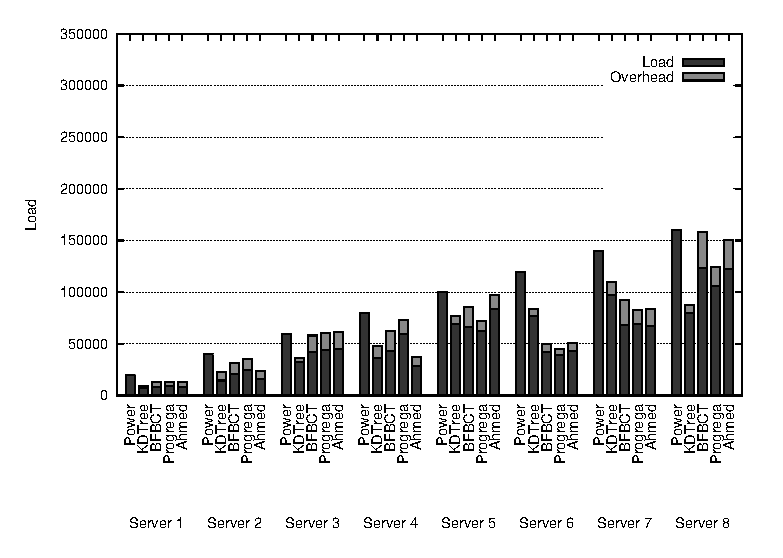
\includegraphics[width=0.49\linewidth]{images/distribution_uniform}
	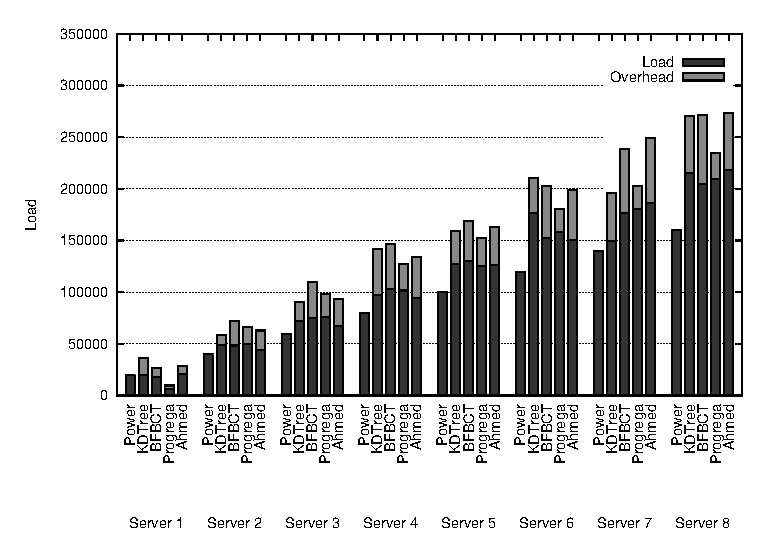
\includegraphics[width=0.49\linewidth]{images/distribution_hotspots}
	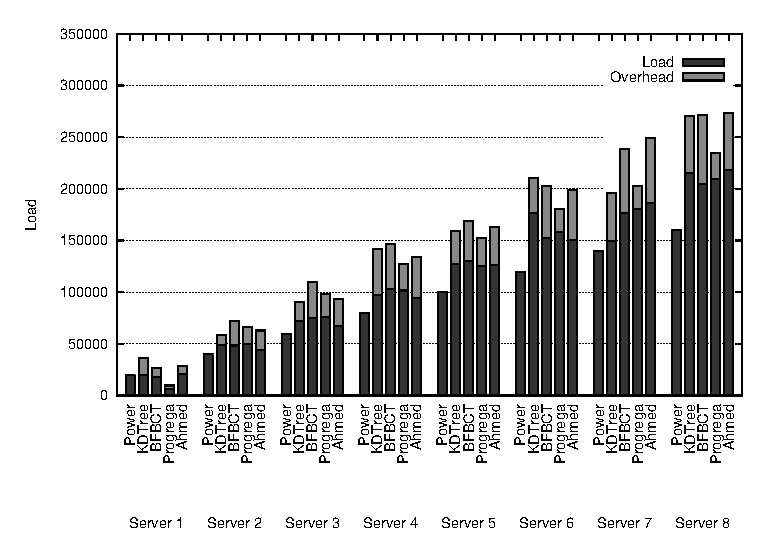
\includegraphics[width=0.49\linewidth]{images/distribution_hotspots}
	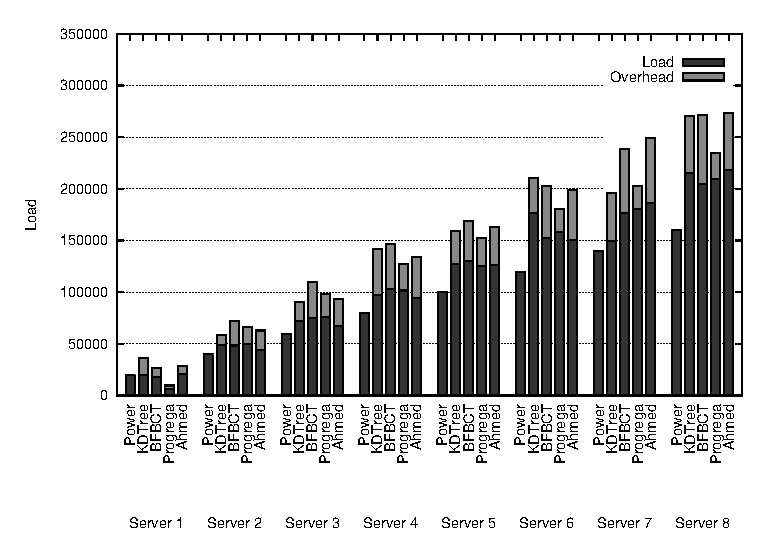
\includegraphics[width=0.49\linewidth]{images/distribution_hotspots}
	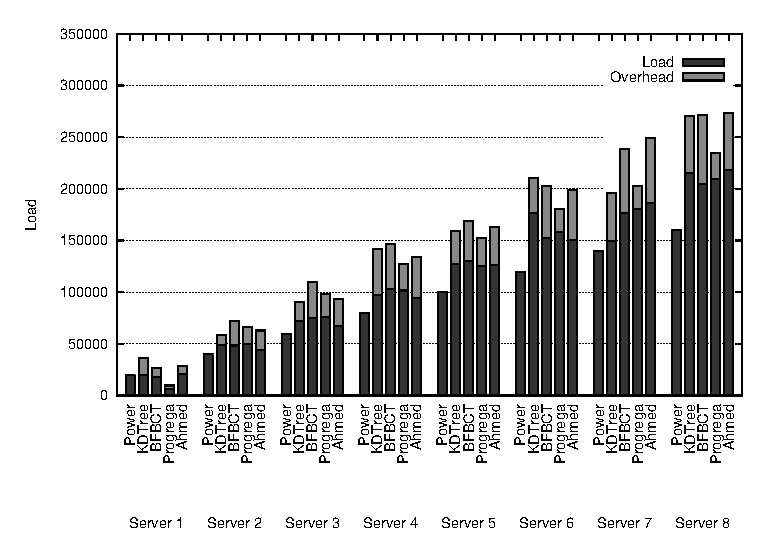
\includegraphics[width=0.49\linewidth]{images/distribution_hotspots}
	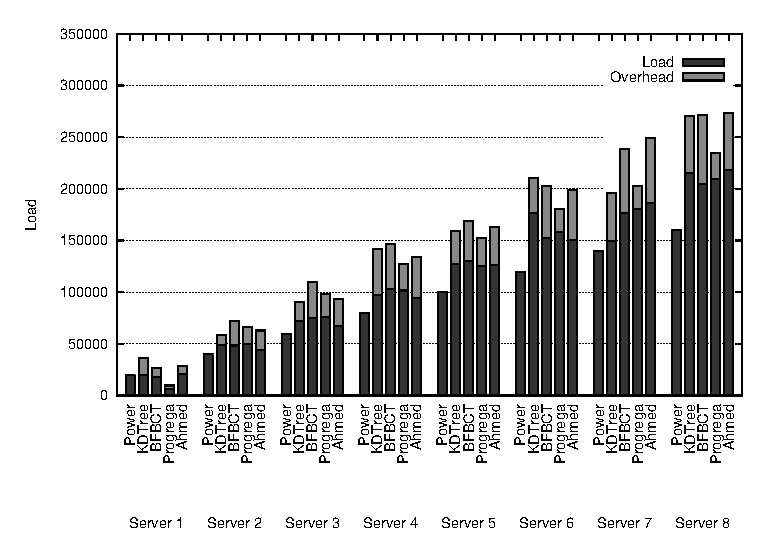
\includegraphics[width=0.49\linewidth]{images/distribution_hotspots}

	\caption{Average load on each server (by algorithm, without hotspots)}
	\label{fig:distribution:uniform}
\end{figure}

%\begin{figure}[!t]
%	\centering
%	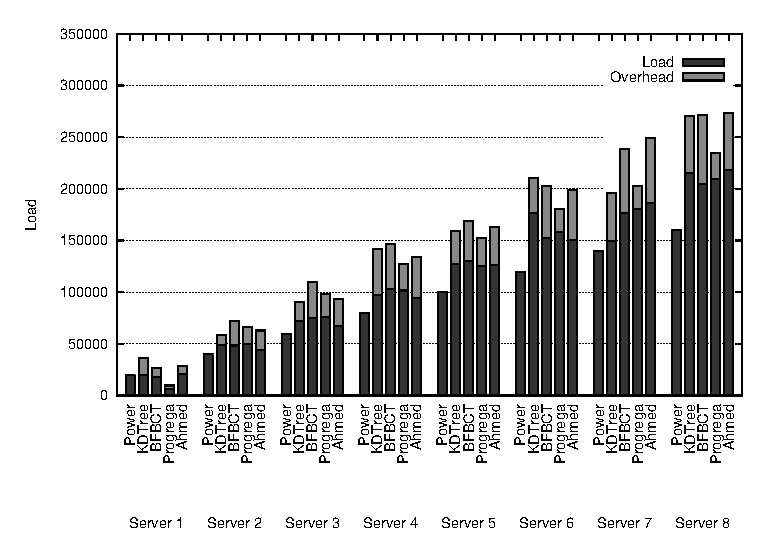
\includegraphics[width=\linewidth]{images/distribution_hotspots}
%	\caption{Average load on each server (by algorithm, with hotspots)}
%	\label{fig:distribution:hotspots}
%\end{figure}

Figures \ref{fig:distribution:uniform} and \ref{fig:distribution:hotspots} present the average load (plus the inter-server communication overhead) on each server, for each algorithm tested. The first figure shows the values in a situation without hotspots and, therefore, a smaller total load. The second, in turn, presents the load distribution when the server system is overloaded. We can see, in Figure \ref{fig:distribution:uniform}, that all algorithms have met the objective of keeping the load on each server less than or equal to its capacity, when the system has sufficient resources to do so. In Figure \ref{fig:distribution:hotspots}, it is demonstrated that all the algorithms managed to dilute -- in a more or less proportional manner -- the load excess on the servers. It is important to observe, however, that the load shown in Figure \ref{fig:distribution:hotspots} is only theoretical. Each server will perform some kind of ``graceful degradation'' in order to keep the load under its capacity. For example, the update frequency might be reduced and access to the game could be denied for new players attempting to join, which is a common practice in most MMOGs.

\begin{figure}[!t]
	\centering
	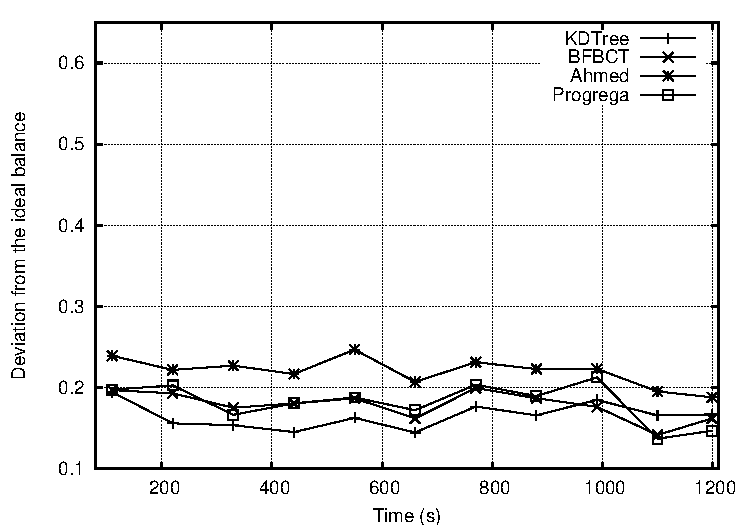
\includegraphics[width=0.49\linewidth]{images/usagedeviation_uniform}
		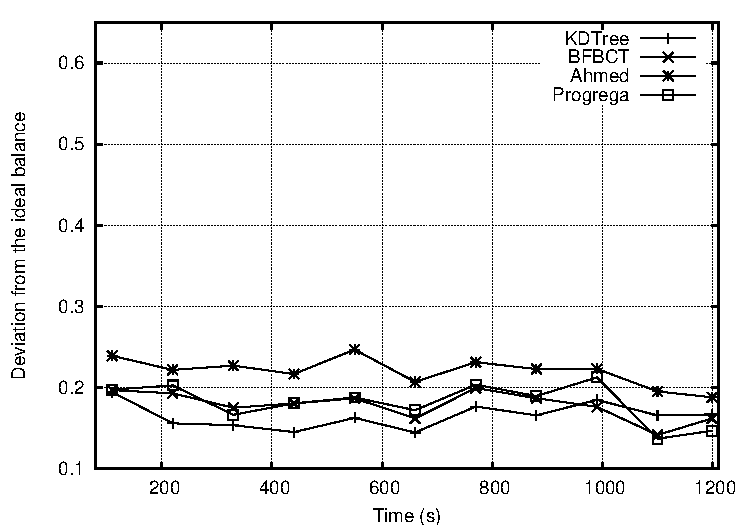
\includegraphics[width=0.49\linewidth]{images/usagedeviation_uniform}
			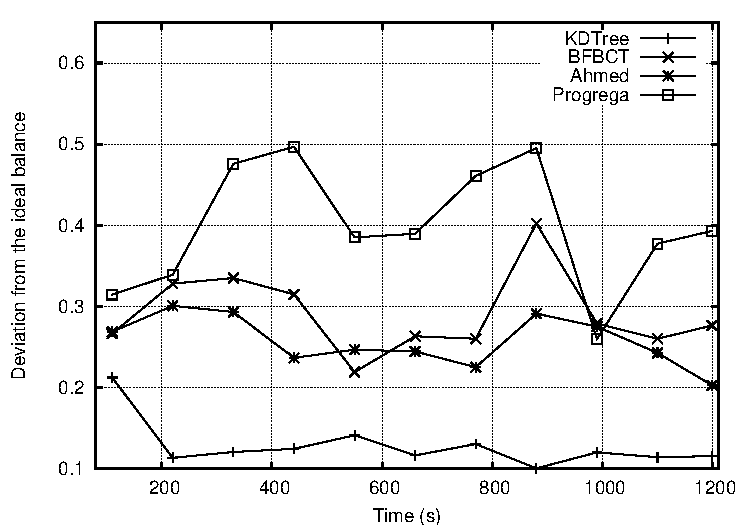
\includegraphics[width=0.49\linewidth]{images/usagedeviation_hotspots}
	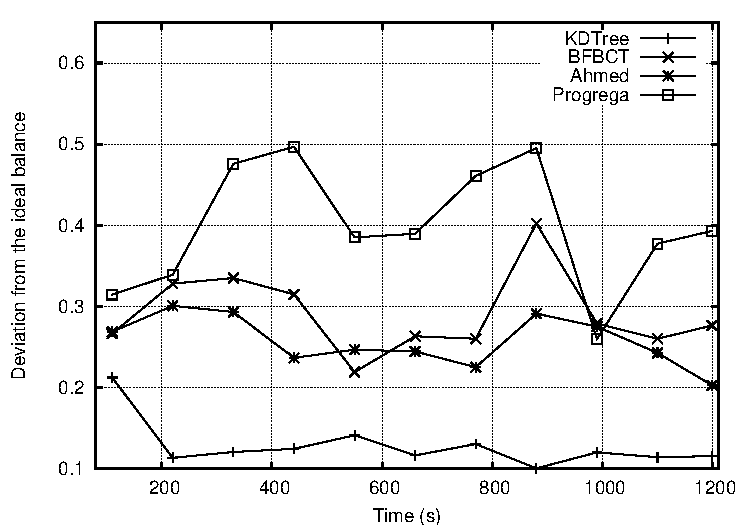
\includegraphics[width=0.49\linewidth]{images/usagedeviation_hotspots}
			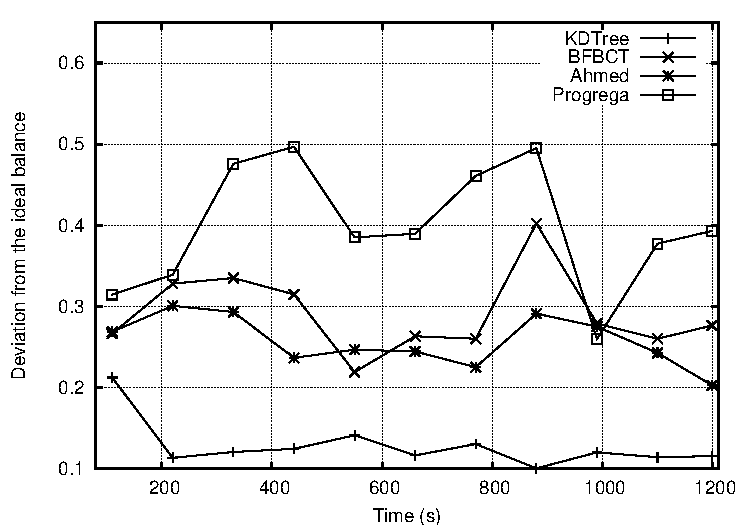
\includegraphics[width=0.49\linewidth]{images/usagedeviation_hotspots}
	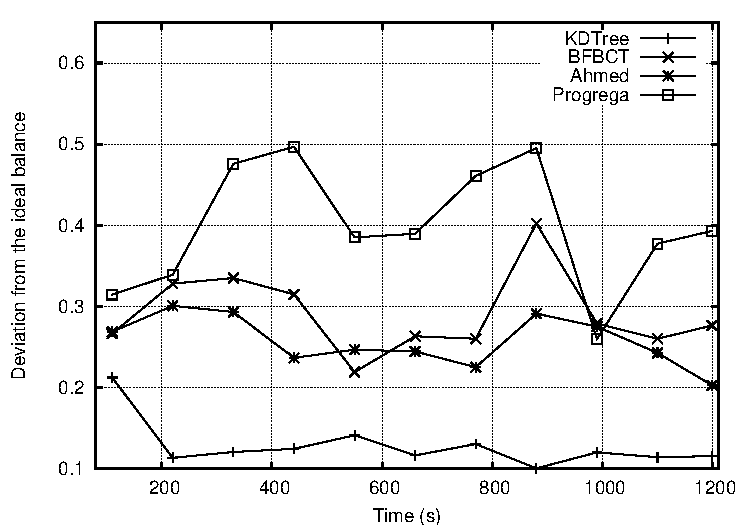
\includegraphics[width=0.49\linewidth]{images/usagedeviation_hotspots}



	\caption{Average deviation of the ideal balance of the servers (without hotspots)}
	\label{fig:usagedeviation:uniform}
\end{figure}

%\begin{figure}[!t]
%	\centering

%	\caption{Average deviation of the ideal balance of the servers (with hotspots)}
%	\label{fig:usagedeviation:hotspots}
%\end{figure}

In figures \ref{fig:usagedeviation:uniform} and \ref{fig:usagedeviation:hotspots}, it is shown how much the balance generated by each algorithm deviates from an ideal balance -- that is, how much, on the average, the load on the servers deviate from a value exactly proportional to the capacity of each one of them -- over time. It is possible to observe that, in both situations -- with and without hotspots -- the algorithm that uses the kd-tree has the least deviation. This is the due to the fine granularity of its distribution, which, unlike the other approaches tested, is not limited by the size of a cell. In the situation with hotspots, the algorithm that uses the kd-tree is particularly effective, because rebalance is needed. In a situation where the system has more resources than necessary, the proportionality of the distribution is not as important: it is enough that each server manages a load smaller than its capacity.

\begin{figure}[!t]
	\centering
	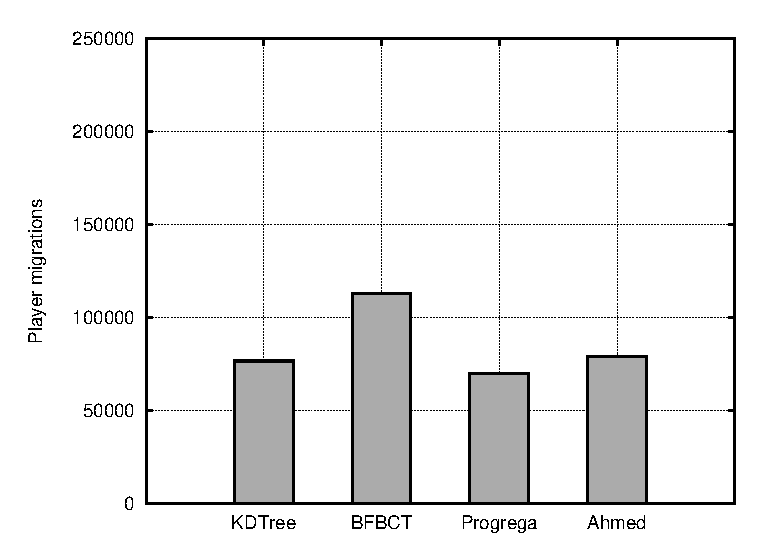
\includegraphics[width=0.49\linewidth]{images/migrations_uniform}
	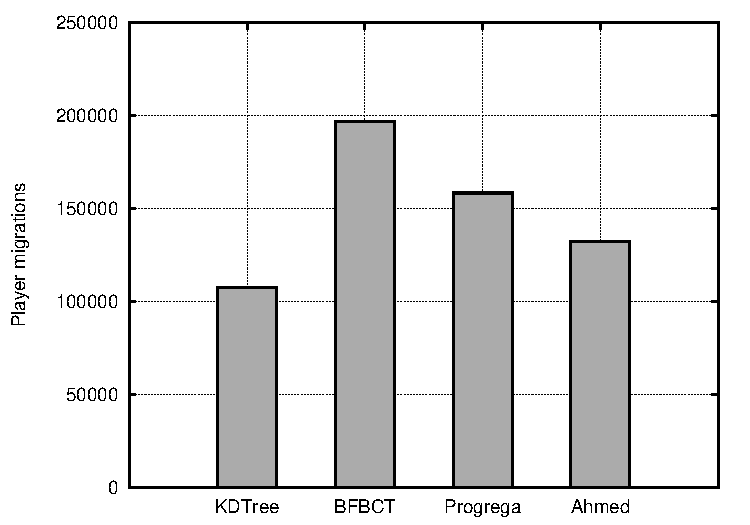
\includegraphics[width=0.49\linewidth]{images/migrations_hotspots}
	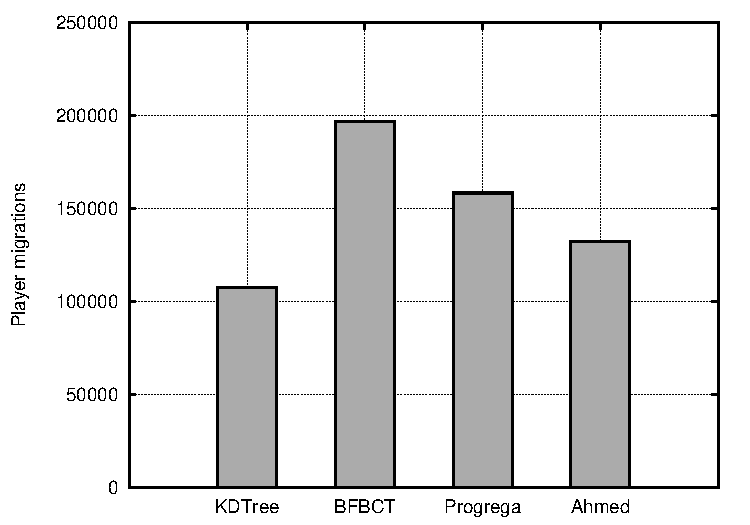
\includegraphics[width=0.49\linewidth]{images/migrations_hotspots}
	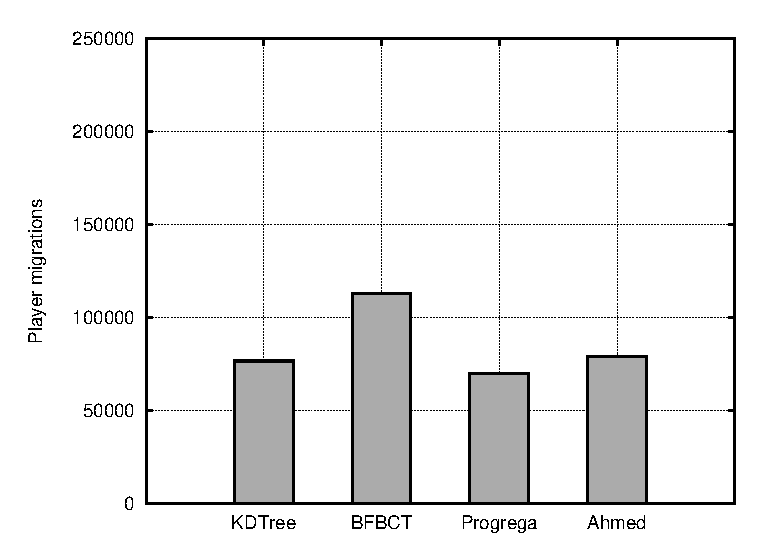
\includegraphics[width=0.49\linewidth]{images/migrations_uniform}
	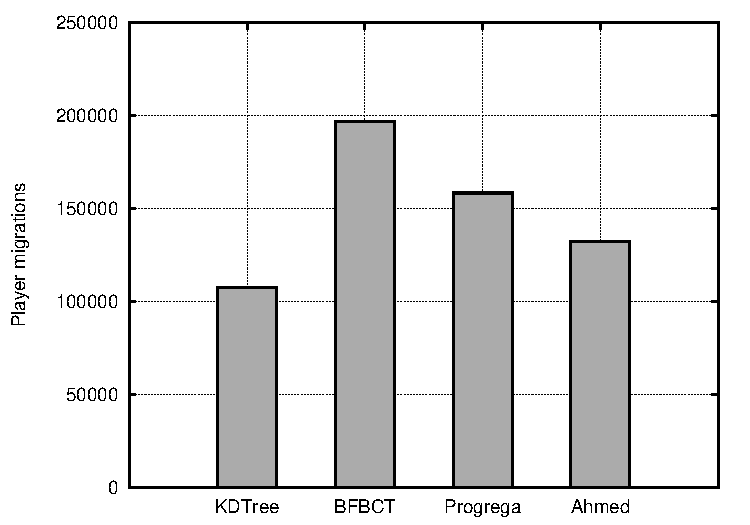
\includegraphics[width=0.49\linewidth]{images/migrations_hotspots}
	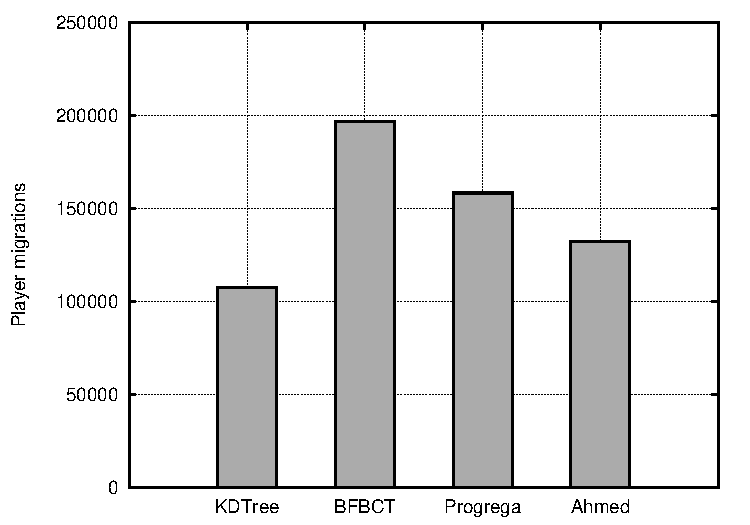
\includegraphics[width=0.49\linewidth]{images/migrations_hotspots}



	\caption{Player migrations between servers (without hotspots)}
	\label{fig:migrations:uniform}
\end{figure}

%\begin{figure}[!t]
%	\centering
%	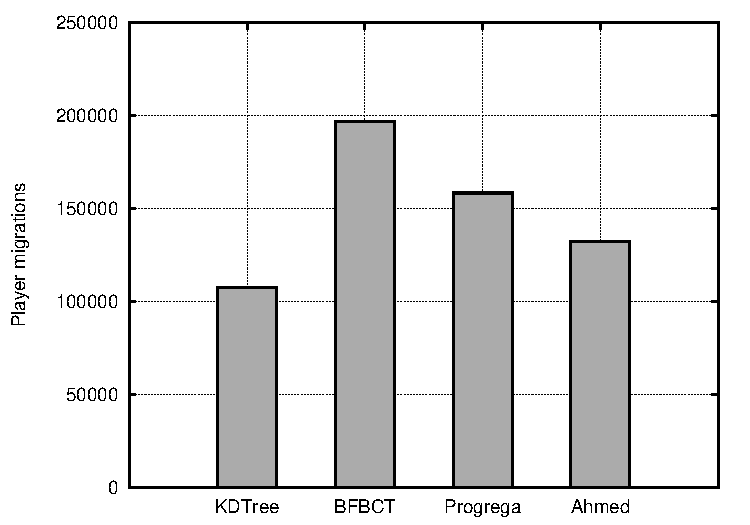
\includegraphics[width=0.8\linewidth]{images/migrations_hotspots}
%	\caption{Player migrations between servers (with hotspots)}
%	\label{fig:migrations:hotspots}
%\end{figure}

Regarding player migrations between servers, all the algorithms -- except BFBCT -- had a similar number of user migrations in the absence of hotspots (Figure \ref{fig:migrations:uniform}). This happens because the load of the game is less than the total capacity of the server system, which required less rebalancing and, thus, caused less migrations of players between servers. Figure \ref{fig:migrations:hotspots}, however, demonstrates that the algorithm that uses the kd-tree had a significantly lower number of user migrations than the other approaches. This is due, in the first place, to the fact that the regions defined by the leaf nodes of the kd-tree are necessarily contiguous, and each server was linked to only one leaf node. An avatar moving across the environment divided into very fragmented regions constantly crosses the borders between these regions and causes, therefore, its player to migrate from server to server repeatedly. Another reason for this result is that each rebalancing executed with the kd-tree gets much closer to an ideal distribution than the cell-based algorithms -- again, thanks to the finer granularity of the kd-tree based distribution --, requiring less future rebalancing and, thus, causing less player migrations.

\begin{figure}[!t]
	\centering
	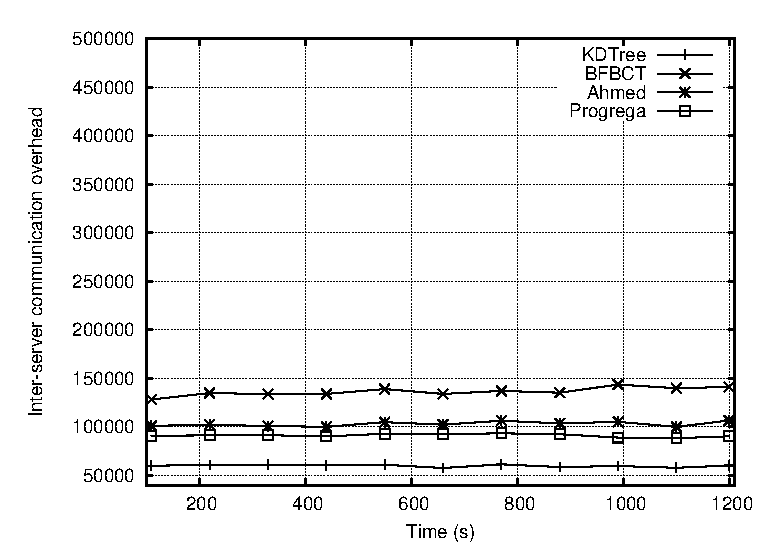
\includegraphics[width=0.49\linewidth]{images/overhead_uniform}
	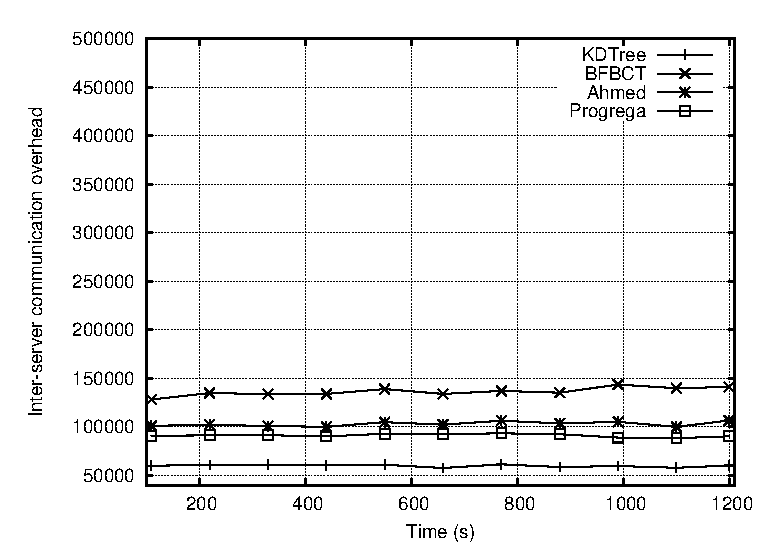
\includegraphics[width=0.49\linewidth]{images/overhead_uniform}
	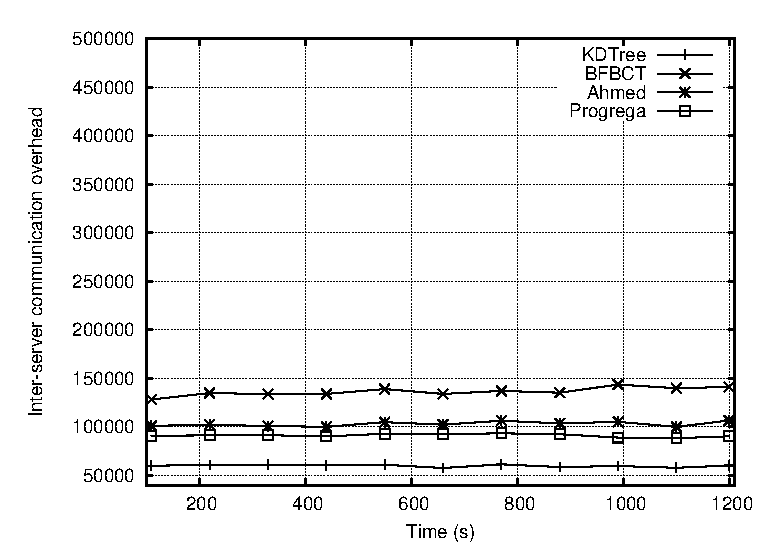
\includegraphics[width=0.49\linewidth]{images/overhead_uniform}
	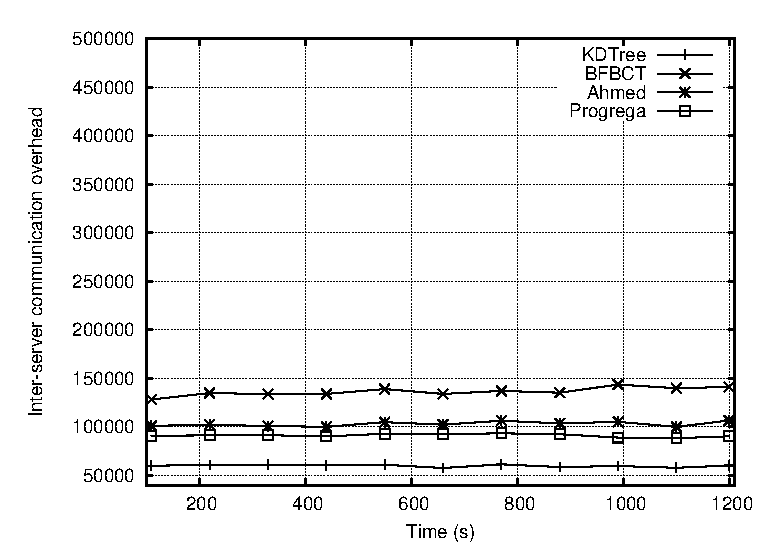
\includegraphics[width=0.49\linewidth]{images/overhead_uniform}
	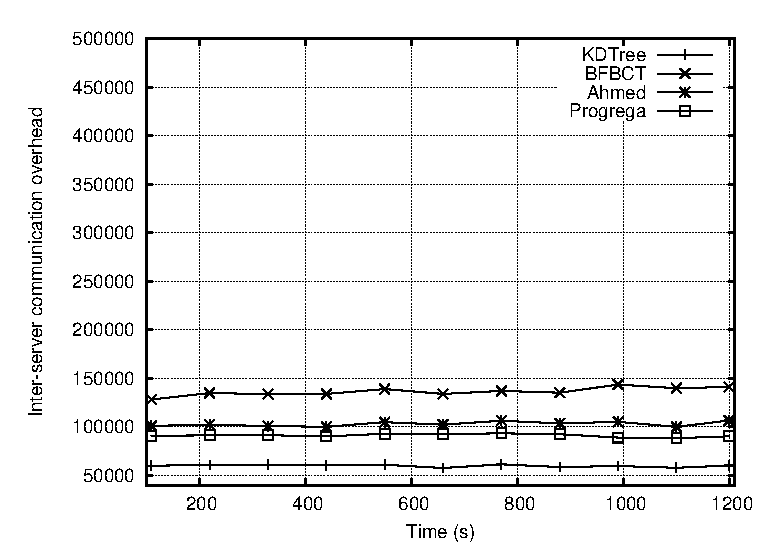
\includegraphics[width=0.49\linewidth]{images/overhead_uniform}
	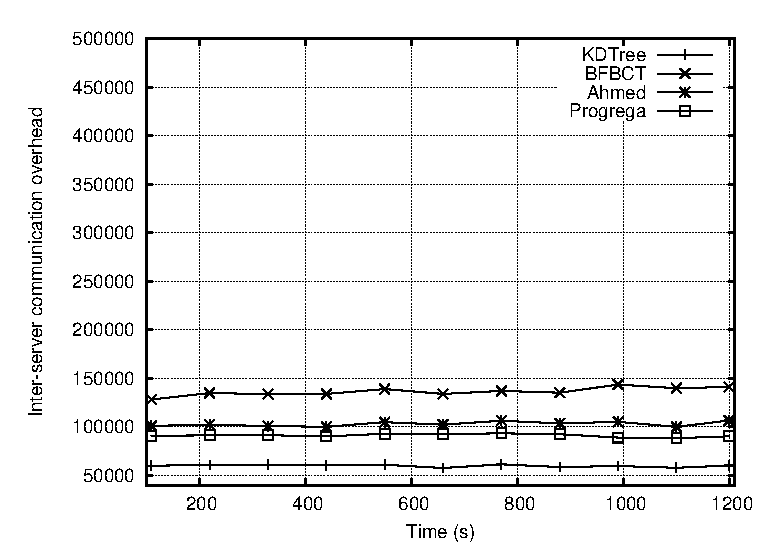
\includegraphics[width=0.49\linewidth]{images/overhead_uniform}

	\caption{Inter-server communication for each algorithm over time (without hotspots)}
	\label{fig:overhead:uniform}
\end{figure}

%\begin{figure}[!t]
%	\centering
%	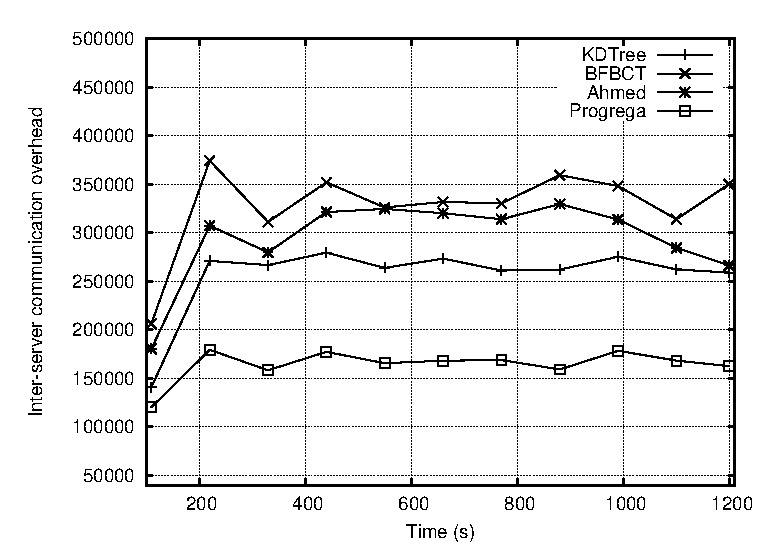
\includegraphics[width=0.8\linewidth]{images/overhead_hotspots}
%	\caption{Inter-server communication for each algorithm over time (with hotspots)}
%	\label{fig:overhead:hotspots}
%\end{figure}

Finally, it is shown the amount of communication between servers for each simulated algorithm, over time. In Figure \ref{fig:overhead:uniform}, all algorithms have similar results, and the one which uses the kd-tree is slightly better than the others. This is also explained by the fact that the regions are contiguous, minimizing the number of boundaries between them and, consequently, reducing the probability of occurring interactions between pairs of avatars, each one in a different region. In Figure \ref{fig:overhead:hotspots}, it is possible to see that the inter-server communication caused by Progrega was considerably lower than all the others in a situation of system overload. The reason for this is that its main goal -- besides balancing the load -- is precisely to reduce the communication between servers. However, even not considering the additional cost, the algorithm that uses the kd-tree got second place in this criterion.

\section{Conclusions}
\label{sec:conc}

In this work, we proposed the use of a kd-tree to partition the virtual environment of MMOGs and perform the load balancing of servers by recursively adjusting the split coordinates stored in its nodes. One of the conclusions reached was that the use of kd-trees to make this partitioning allows a fine granularity of the load distribution, while the readjustment of the regions becomes simpler -- by recursively traversing the tree -- than the common approaches, based on cells and/or graph partitioning.

The finer granularity allows for a better balancing, so that the load assigned to each server is close to the ideal value that should be assigned to it. This better balance also helped to reduce the number of migrations, by performing less rebalancing operations. The fact that the regions defined by the kd-tree are necessarily contiguous was one of the factors that contributed to the results of the proposed algorithm, which was better than the other algorithms simulated in most of the criteria considered.

In conclusion, it was possible to use methods that can reduce the complexity of each rebalancing operation. This is due, first, to the reduction of the number of operations for calculating the relevance between pairs of avatars by sweeping a sorted avatar list and, secondly, to keeping at each server an avatar list already sorted in both dimensions, saving the time that would be spent on sorting the avatars when they were received by the server executing the rebalance.



\subsection{Acknowledgments}

The development of this work has been supported by the National Research Council (CNPq) and by the Coordination for Improvement of the Higher Education Personnel (CAPES).

\bibliographystyle{acmtrans}
\bibliography{kdtree}
\begin{received}
Received February 1986;
November 1993;
accepted January 1996
\end{received}

%{\let\setcounter\mycounter
%	\elecappendix
%}

\medskip

\end{document}




